
\synctex=1

\documentclass[11pt]{report}
\usepackage[lmargin=30pt,rmargin=115pt,tmargin=70pt,bmargin=70pt,marginparwidth=110pt,marginparsep=5pt,a4paper]{geometry}
\usepackage{amssymb}
\usepackage{hyperref}
%\usepackage[tiny,compact]{titlesec}
\usepackage{graphicx}

\usepackage{booktabs}


\usepackage{wrapfig}
\usepackage{textcomp}
\usepackage{bold-extra}
\usepackage{tikz}
\usepackage{qtree}
\usepackage{tikz-qtree}
\usepackage{expex}


\usetikzlibrary{positioning,decorations.pathmorphing,arrows.meta,decorations.text}
\tikzset{snake it/.style={decorate, decoration=snake}}
\usetikzlibrary{calc, shapes, backgrounds,angles,quotes,tikzmark}
\usepackage{afterpage}
\usepackage{verbatim}
\usepackage{array}
\usepackage{multirow}
%\usepackage{hanging}
\usepackage{supertabular}
\usepackage{mathtools}
\usepackage[all]{xy}
\usepackage{ot-tableau}

\usepackage{paralist} 
\usepackage[labelsep=period,labelfont=bf]{caption}
\usepackage{subcaption}
\usepackage{fancyhdr} 
\usepackage{sectsty}
%\allsectionsfont{\sffamily\mdseries\upshape} 
\usepackage{float}
\usepackage[nottoc,notlof,notlot]{tocbibind} 
\usepackage[titles,subfigure]{tocloft} 
\usepackage{setspace}
%\usepackage[colorinlistoftodos]{todonotes}
\usepackage{xcolor}

\definecolor{blech}{rgb}{.78,.78.,.62}
\definecolor{ochre}{cmyk}{0, .42, .83, .20}
\definecolor{shadecolor}{cmyk}{.08,.08,.1,.12}
%\usepackage[explicit]{titlesec}
%\usepackage{type1cm}
%\usepackage{xcolor}

\usepackage{xltxtra} % Loads fontspec, xunicode, metalogo, fxltx2e, and some extra customizations for XeLaTeX
%\defaultfontfeatures{Mapping=tex-text} % to support TeX conventions like ``---''
\defaultfontfeatures{Mapping=tex-text}
\setmainfont{Cambria}

\usepackage[sort]{natbib}
\bibliographystyle{apa}
\bibpunct[:]{(}{)}{,}{a}{}{,}

%\usepackage{gb4e} \let\eachwordone=\it %\let\eachwordthree=\sf


\makeatletter
\def\@xfootnote[#1]{%
	\protected@xdef\@thefnmark{#1}%
	\@footnotemark\@footnotetext}
\makeatother

\pagestyle{fancy}
\fancyhf{}
\rhead{\footnotesize %Josh Phillips
	\hspace{2cm}\textbf{\thepage}}
\rfoot{}

\renewcommand{\headrulewidth}{0pt} 
\newcommand{\rowgroup}[1]{\hspace{-1em}#1}
\usepackage{stmaryrd}
\newcommand{\denote}[1]{\mbox{$[\![\mbox{#1}]\!]$}}
\newcommand{\denotn}[1]{\mbox{\llbracket\mbox{#1}\rrbracket}}

\newcommand{\mcom}[1]
{\marginpar{\color{black}\raggedleft\raggedright\hspace{0pt}\linespread{0.9}\footnotesize{#1}}}
\newcommand{\cb}[1]
{\marginpar{\color{orange}\raggedleft\raggedright\hspace{0pt}\linespread{0.9}\footnotesize{#1}}}
\newcommand{\hk}[1]
{\marginpar{\color{purple}\raggedleft\raggedright\hspace{0pt}\linespread{0.9}\footnotesize{#1}}}
\newcommand{\note}[1]{{ }\mcom{Note}\textbf{#1}}


\newcommand{\glem}[1]
{\MakeUppercase{\scriptsize{\textbf{#1}}}}

\newcommand{\exem}[1]
{\textit{\textbf{#1}}}

\usepackage{framed}
\usepackage{wrapfig}


\date{}
\begin{document}
	
%\part{Yolŋu Matha intensionality}


\vspace*{\fill}
\sl Drawing on data from Yolŋu~Matha, a subfamily of Pama-Nyungan spoken in central- and eastern Arnhem Land, this Part of the Dissertation provides an amphichronic description and analysis of the Yolŋu~Matha verbal paradigm and a discussion of the linguistic devices that speakers use for displacement: temporal and modal displacement.

Yolŋu Matha is a language family spoken in north-central and -eastern Arnhem Land. \mcom{Xref here to introductory chapter/s}. As explained in Chapter \ref{ecology}, subgrouping of the family remains somewhat controversial, but most treatments understand the it as containing six languages with thirty or so `clan-lects' distributed between them. For the purposes of this prospectus, I will make reference to the closely related Western varieties of Djambarrpuyŋu (\texttt{[djr]} Dhuwal) and Gupapuyŋu (\texttt{[guf]} Dhuwala), slightly further afield Wangurri (\texttt{[dhg]} Dhaŋu) and Southern variety Ritharrŋu \texttt{[rit]}; the varieties for which there is the most significant amount of presently available documentation.

\textbf{Chapter \ref{descY}} contains a general description of the language ecology of Yolŋu Matha and patterns of verbal inflection in Yolŋu varieties, paying particular attention to Djambarrpuyŋu, how it diverges to Djinba, Ritharrŋu and Wangurri, and the puzzles that these paradigms pose for theories of tense and modality.

\textbf{Chapter \ref{anY}} proposes a formal treatment and analysis of temporal and modal expression in synchronic Yolŋu varieties.

\textbf{Chapter \ref{diaY} }foregrounds `diachronic thinking' about the comparative Yolŋu data presented here and considers: {\em What might the paths of change and synchronic variation in Yolŋu Matha suggest about the cognitive implementation of displacement operators?}
\vfill

\upshape 

\chapter{The Yolŋu~Matha verbal paradigm}\label{descY}



The verbal inflectional paradigms of contemporary Yolŋu languages can be reconstructed to proto-Yolŋu (\textit{e.g.} Bowern 2009). Notwithstanding this demonstrated cognacy, there is significant cross-linguistic variation reported in the distributions and `meanings' associated with the varieties' cognate inflectional categories. Where eastern and southern language varieties are described as having `basic tense categories' that are `semantically straightforward' (\textit{e.g.} \citealt{Heath1980} on Ritharrŋu:74\textit{ff}), an adequate treatment of the morphosemantics of tense marking in the related Yolŋu languages spoken in western Arnhem Land appears to be much more elusive, notwithstanding the nuanced and detailed descriptions in \citealt{Wilkinson1991} and \citealt{McLellan1992}.


\mcom{Do I want to talk at this point about adopting a particular (probably realizational) morphological theory?} In this chapter, I provide description of verbal inflection across a number of Yolŋu varieties on the basis of data from existing descriptive works (published grammars and related publications) in addition to novel field data collected by the author. For reasons that will become clear, I pay particular attention to the \textit{Dhawu} variety Djambarrpuyŋu (Dhuwal) and mutually the intelligible \textit{Yirritja} variety Gupapuyŋu (Dhuwala). The verbal inflectional system for this language is described in §\ref{djr}.


\mcom{Will work on acquiring a nicer-looking map. Also it may/probably will turn out this this is better placed in Chapter 1 (the  basic introduction to Arnhem Land.)}\begin{figure}[h]
	\centering\caption{Traditional language communities in Northern Australia \citep{Horton1996}.\\\textbf{Inset. }Northeast Arnhem land (colourised from \citealt[2]{Wilkinson1991}. Yellow shading indicates the \textit{Yolŋu Wäŋa} (homeland). Brown and green circles indicate the contemporary distribution of Yolŋu languages investigated. Purple circling indicates the neighbouring (but genetically unrelated) Maningrida language family.}	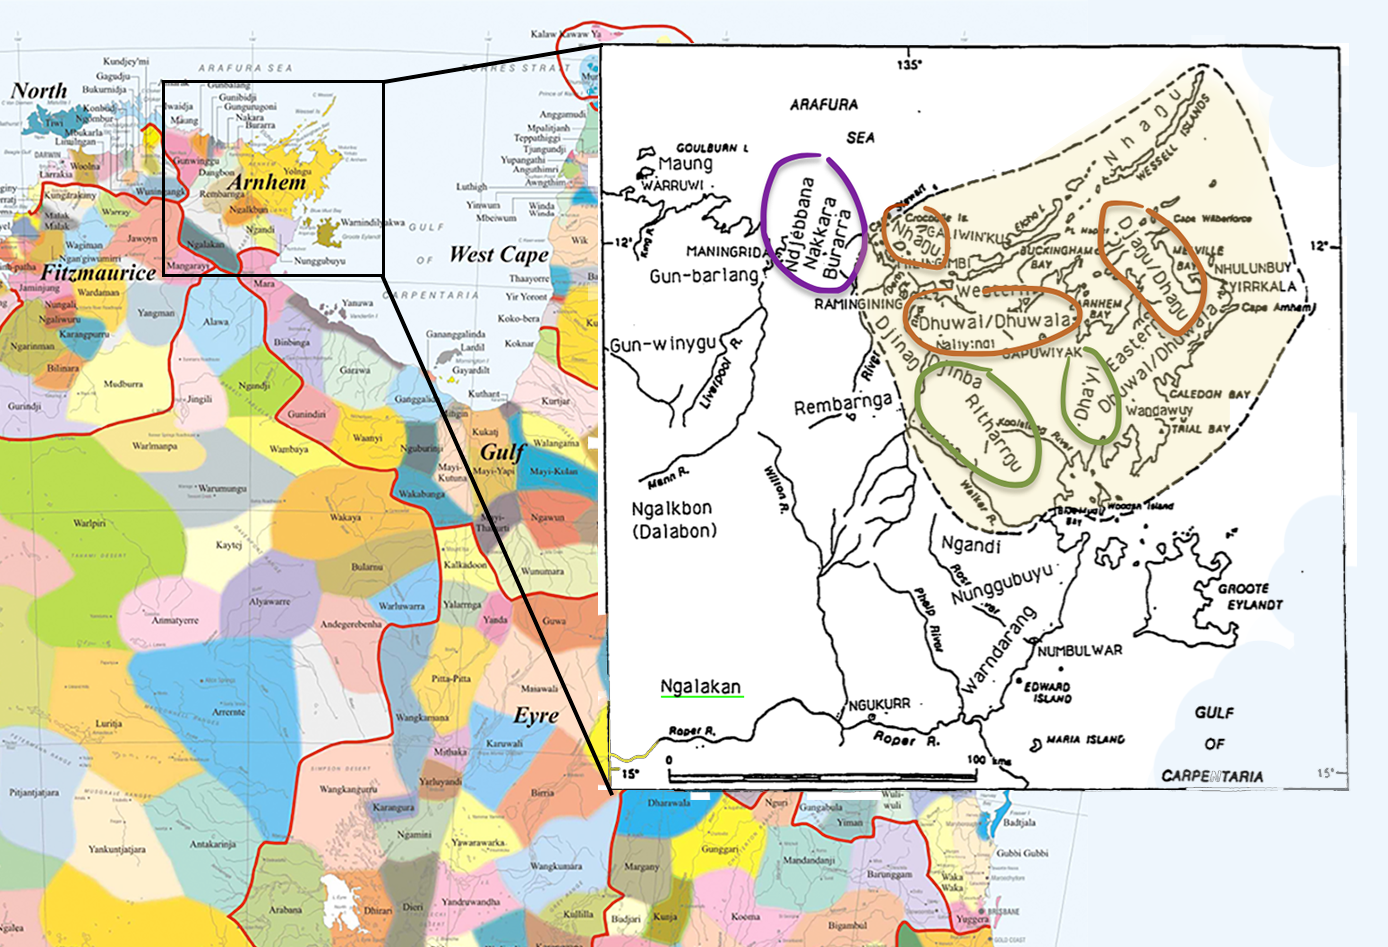
\includegraphics[width=0.7\textwidth]{AustralianLangsCropped.png}\label{map}
\end{figure}




\section{Djambarrpuyŋu \& Gupapuyŋu}\label{djr}

TMA distinctions in Dhuwal(a) are encoded in a paradigm that disinguishes four `inflections', which are cognate with a number proto-Yolŋu inflections according to the reconstructions provided by \citet{Bowern2009}. Work on Dhuwal and Dhuwala varieties (notably \citealt{Wilkinson1991,Lowe1996}) has eschewed a metalinguistic gloss for these inflections, given the ostensible non-unifiability of their semantics. Both authors appeal to an arbitrary numbering system for the four ``inflections'', which I follow in this section. In addition to these inflections, the expressive burden of encoding TMA relations is shared by a (closed) class of auxiliaries, which appear to interact with the verbal paradigm. 

Further complicating the exposition of this, is the fact that there are a number of \textit{conjugation (sub)classes}: 9 according to \citet{Lowe1996} for Gupapuyŋu, 3 larger classes each with a number of subclasses in addition to ``non-inflecting'' and (semi-)irregular categories for the closer description in \citet{Wilkinson1991}.


\subsection{The verbal inflections}

As mentioned above, Dhuwal(a) varieties make use of a verbal paradigm with four inflectional distinctions. As discussed in Chapter \ref{ecology}, varieties of Dhuwal-Dhuwala are mutually intelligible, the primary distinction resulting from a productive apocope rule \citep[51]{Morphy1977}. The formal consequences of Dhuwal apocope on the verbal paradigm are shown in Table \ref{djr-pdm-exx} below. The table gives examples of the verb paradigm for each of the major Djambarrpuyŋu conjugation classes as described by \citet[306ff]{Wilkinson1991} (parentheses give the corresponding verb group number assigned by \citet{Lowe1996} for Gupapuyŋu.)

\begin{table}[h]\centering
	\begin{tabular}{ll|llll}
		\textbf{Class} & \textbf{\textit{Example}} & \textbf{I} & \textbf{II} & \textbf{III} & \textbf{IV}\\\midrule
		$\boldsymbol\emptyset$  (2)& \textit{marrtji} `go' & \textit{marrtji}& \textit{marrtji} & \textit{marrtji\textbf{n(a)}} & \textit{marrtji\textbf{nha}}\\
		\textbf{N} (5) & \textit{ḻupthu\textbf{n}} `wash' &\textit{ḻuphtu\textbf{n}} & \textit{ḻupthu\textbf{rr(u)}} & \textit{ḻupthu\textbf{rr(una)}} & \textit{ḻupthu\textbf{na}}\\
		 \textbf{Ŋ} (7)  & \textit{nhäma} `see' & \textit{nhä\textbf{ma}} & \textit{nhä\textbf{ŋu}} & \textit{nhä\textbf{ŋal(a)}} & \textit{nhä\textbf{nha}}\\
				\end{tabular}
			\caption{Examples of the paradigm of four morphological TMA inflections in Djambarrpuyŋu \texttt{[djr]} and (Gupapuyŋu \texttt{[guf]}). \texttt{djr} data from \citet{Wilkinson1991}, \texttt{guf} data from \citet{Gupapuyngu2016}.} \label{djr-pdm-exx}
\end{table}

In the first paragraph of this section, I alluded to Beulah Lowe's eschewal of a ``semantic description'' for each of the four inflectional classes. Melanie Wilkinson follows this system in her 1991 grammar and I will follow them here. Below I provide examples of the functional domains of each of the four inflections in Dhuwal-Dhuwala. Inflections are glossed with the bold-faced Roman numerals given in Table \ref{djr-pdm-exx}.

\subsubsection{The Primary inflection}

\subsubsection{The Secondary inflection}

\subsubsection{The Tertiary inflection}

\subsubsection{The Quaternary inflection}


\subsection{Aspectual auxiliaries}

\subsection{Modal auxiliaries}


\chapter{The Yolŋu language of intensionality}\label{anY}
\chapter{Variation, change \& `design principles'}\label{diaY}

\vfill\bibliographystyle{apa}\bibliography{../../FullBiblio.bib}

\end{document}